\documentclass[11pt]{article}
\usepackage{graphicx} % Required for inserting images

% set up the packages for the references
\usepackage[
backend=biber, sorting=none, style=science, url=false, isbn=false, note=false, pages=false, language=false
]{biblatex}

% for references and links
\usepackage{hyperref}

% for setting up figures
\usepackage{subfigure}
\usepackage{multirow}

% package for margin spacing
\usepackage[margin=1in,inner=1in]{geometry}
\geometry{top=0.5in}

% package for math stuff
\usepackage{algorithmic}
\usepackage{algorithm}
\usepackage{mathtools}
\usepackage{amssymb}
\usepackage{amsmath}

\addbibresource{refs.bib}

\title{Technical Report: \\
\large Hydro-electric power optimization service}
\author{Student number: 30832950}
\date{March 2023}

\begin{document}

\maketitle

\section*{Introduction}

The 2018 Japan floods, which occured between late June and mid-July 2018, were caused by a series of heavy rainfall events and primarily affected the Shikoku and Honshu areas \parencite{wiki:2018_Japan_floods}. The heavy rainfall caused landslides and widespread flooding, resulting in the loss of lives, as well as extensive damage to infrastructure. Among the facilities affected were hydroelectric power stations, which had to adapt to significant operational challenges in order to manage the reservoir levels. In this report we consider how climate data, such as reanalysis products and subseasonal to seasonal (S2S) forecasts, can be used to inform the operational management of a hydroelectric power station. We consider the 2018 Japan floods as a case study to explore this, as S2S forecasts had predicted the period of heavy precipitation well in advance. This meant that dam operators were in a position to respond to this warning and had to minimise risk while also meeting multiple constraints. For a hydroelectric power station to generate electricity, there must be sufficient head of water behind the dam to maintain a continuous flow of water through turbines. In addition, water levels in the reservoir must be kept within a safe range, to avoid running out of water during the summer and prevent the water levels from becoming too high and overtopping. As a result, the 2018 Japan floods can be used as a case study to demonstrate the opportunities and limitations of climate services.\\

First, this report will consider the climate data used in this retrospective climate service. Then the modelling approaches used to explore this service will be described. The results of this study will then be presented, using figures and statistics, along with answers to key research questions. Then, in the discussion, we will consider the limitations of the methodology (and data) presented here and propose potential areas for future development. The report will then conclude with a summary of our findings. 

\section*{Data}

The climate data used in this study are reanalysis and S2S forecasts.

\subsection*{Reanalysis}

% reference for this maybe?

Reanalysis data combines observations from a global network with short-range weather forecasts to provide a globally complete, continuous best estimate of the past weather and climate \parencite{ecmwf:reanalysis}. Here, we use the ERA5 dataset from the European Center for Medium-Range Weather Forecasts (ECMWF), which provides hourly estimates of relevant variables on a 0.1 degree grid (around 30km). This dataset is used as our observations due to its high resolution and spatial coverage. As we only require daily accumulated runoff data, the temporal resolution is actually higher than is necessary. 

\subsection*{S2S forecasts}

% perhaps a reference for this?

Subseasonal to seasonal (S2S) forecasts bridge the gap between short-term synoptic forecasts and longer-term seasonal and decadal (and beyond) projections. These cover a timeframe from about 2 weeks to 3 months and provide information on the likely evolution of large-scale conditions during that period \parencite{s2s:homepage}. Specifically we use probablistic S2S forecasts from ECMWF, which contain 50 ensemble members each initialised with perturbations to the initial conditions. These subseasonal forecasts are made every 3-4 days and predict the evolution of conditions over the next 46 days. As they are longer-range forecasts, the resolution is more coarse than the reanalysis product with a 1.5 degree grid (greater than 100km). Therefore, in order to make comparisons between the S2S and reanalysis data, the reanalyis data must be downscaled to the lower-resolution grid of the S2S forecast data. Despite this, the probabilistic subseasonal forecasts from ECMWF are suitable for our needs as they are made at regular intervals and are at a suitable resolution to resolve the accumulated runoff in the study region.

\section*{Methods}

% describe the calculations you performed with the data
% mathematically and in words
% and any important considerations for your calculations
% refer to lecture notes for guidance on how to approach such problems
% and best practice

\subsection*{Dam optimization model}

In this study we use a dam optimization model based on \parencite{hirsch2014hydro} to predict the most likely operational pathway for the dam when given the runoff time series as input. This model produces the solution for the optimum flow rate and resulting power generation rate as output. The model is set up with the characteristics and constraints for our study area; Tokuyama Dam which is located in southwestern Honshu and our catchment which is defined by the grid box 34-36 $^{\circ}$N and 135-137 $^{\circ}$E.\\

The model is defined by the following:

\begin{equation}
    \frac{dS}{dt} = I - W - R
    \label{simple_ODE}
\end{equation}

Where
\begin{description}
    \item S is the reservoir storage volume (m$^3$);
    \item I is the inflow from the water catchment, which is dependent on the catchment hydrology (m$^3$ s$^{-1}$);
    \item W is the flow rate through the turbines (m$^3$ s$^{-1}$);
    \item R is the relief from from the dam which avoids the turbines (m$^3$ s$^{-1}$).
\end{description}

The power generation rate is dependent on the flow rate through the turbines (W) and the reservoir head (H):

\begin{equation}
    G = \mu \sigma WH
    \label{power_gen}
\end{equation}

Where $\mu$ is a conversion factor to the units of generation rate (MW) and $\sigma$ is the energy conversion efficiency of the hydroelectric plant. The reservoir volume is assumed to be proportional to the head, according to the constant $\kappa = A/2$, where A is the reservoir area.

\begin{equation}
    S = \kappa H
    \label{volume_head}
\end{equation}

This model is run over a period of time using a centred difference scheme for the rate of change of head (H), which is rearranged to give the flow rate through the turbines at time step $n$, $W_n$:

\begin{equation}
    W_n = - \frac{\kappa}{2 \Delta t} \biggl( H_{n+1} - H_{n-1} \biggr) + I_n - R_n
    \label{centred_diff_flowrate}
\end{equation}

Using equation \ref{power_gen}, the centred difference scheme can be expressed as power generated by the dam at time $t_n$ as:

\begin{equation}
    G_n = - \mu \sigma \frac{\kappa}{2 \Delta t} \biggl( H_{n+1} - H_{n-1} \biggr)H_n + \mu \sigma(I_n - R_n) H_n
    \label{centred_diff_powergen}
\end{equation}

The model solves the finite-differences scheme in equation \ref{centred_diff_powergen} to maximise the total power generation over the entire time period ($G_n \forall n$), given the following constraints:

\begin{align*}
    H_{min} \leq H_n \leq H_{max} \\
    W_{min} \leq W_n \leq W_{max}
    \label{constraints_H_W}
\end{align*}

Whereby the water depth must be above the minimum allowed head ($W_{min}$) but beneath the maximum depth ($W_{max}$) and the flow rate must be within a safe operational range.\\

The Tokuyama dam has the following characteristics:\\

\begin{center}
        \begin{tabular}{|p{3cm}|p{6cm}|p{4cm}|} % adjust the widths as needed
            \hline
            Parameter & Name & Value \\ \hline % first row
            $H_{dam}$ & Dam height & 161 m \\ \hline % second row
            $A$ & Reservoir area (specifies $\kappa$) & 13 km$^2$ \\ \hline % third row
            $A_{catch}$ & Catchment area & 254 km$^2$ \\ \hline % fourth row
            $H_{max}$ & Maximum safe head of water at dam & 80.5 m \\ \hline % fifth row
            $H_{min}$ & Minimum safe head of water at dam & 32.5 m \\ \hline % sixth row
            $\tau$ & Reservoir emptying timescale at max flow rate ($W_{max}$) & 180 days \\ \hline % seventh row
            $W_{max}$ & Maximum flow rate: $W_{max} = \kappa/\tau H_{dam}$ & 67.3 m$^3$ s$^{-1}$ \\ \hline % eighth row
            $W_{min}$ & Minimum flow rate through turbines & 6.7 m$^3$ s$^{-1}$ \\ \hline % ninth row
            $R_{max}$ & Maximum flow rate through turbines & 13.5 m$^3$ s$^{-1}$  \\ \hline % tenth row
            $G_{max}$ & Maximum power generation rate by turbines & 153 MW \\ \hline % eleventh row
            $\mu$ & Conversion factor to units of generation rate (MW): $\mu = G_{max}/(\sigma W_{max} H_{dam})$ & 0.015  \\ \hline % twelth row
            $\sigma$ & Energy conversion efficiency of the hydro power plant & 0.9 \\ \hline % thirteenth row
        \end{tabular}
\end{center}

To maximise the power generated ($G_n$) in the solution of equation (\ref{centred_diff_powergen}), our dam optimization model utilizes the \texttt{scipy.optimize.minimize()} function. This uses sequential least squares quadratic programming (SLSQP) to find the optimal value for the reservoir head (x) that minimises the objective function \texttt{gen} and so maximises the negative of the output (\texttt{f}, equivalent to the power generation $G_n$). The optimal values of head (x) are used to calculate the optimum flow rate through the turbines (w) and relief flow (r). The negative value of the objective function (\texttt{f}), which has been maximised using SLSQP, is multiplied by -1 to get the positive value for the time integrated generation for the optimal solution (\texttt{gout}).\\

The purpose of the climate service discussed here is to combine climate information from reanalysis and S2S forecasts with sectoral information from the dam optimization model to provide actionable information in the form of forecasts for optimal dam operation pathways. The methodology used in this study is visualised in figure \ref{fig:climate_service}

\begin{figure}
    \centering
    \scalebox{0.4}{
    \includegraphics{Climate_services_figure_png_cropped.png}}
    \caption{Illustration of the components of this climate service.}
    \label{fig:climate_service}
\end{figure}

\subsection*{Research questions}

To explore the potential applications of climate services to the operational management of a hydroelectric dam in Japan, this study considers six research questions. These questions, and the methods used to answer them, are detailed below.

\begin{enumerate}
    \item Does the simple optimization model return plausible results for flow rate when provided with a time series of inflow data from ERA5? How long a time series of input data is required for stable results (using the default parameter settings)?
        \begin{itemize}
            \item To create a time series of input data for use in the optimization model we use bilinear interpolation to regrid the ERA5 data to a single grid point at the location of the Tokuyama dam (35.63$^\circ$N, 136.48$^\circ$E). The values for this single grid point are interpolated by taking the weighted average of the four nearest grid points.
            \item To test the stability of the dam optimization model for different lengths (and characteristics) of input data, we run the optimization for different time periods in 2017 and 2018, where the 2018 runs include the extreme rainfall event of late June/early July.
        \end{itemize}
    \item How does the model output depend on varying the three parameters: $H_{max}$, $H_{min}$, and $W_{max}$ (depends on timescale, $\tau$)?
        \begin{itemize}
            \item To explore the impacts of varying $W_{max}$ we use a high (low) value of $\tau$ to give a smaller (larger) value for $W_{max}$.
            \item To explore the sensitivity to the range of reservoir head ($H_{range} = H_{max} - H_{min}$) we run the model with a large $H_{range}$ and a small $H_{range}$.
        \end{itemize}
    \item How do the statistics of water runoff in the (uncalibrated) S2S forecast data compare to the runoff in ERA5 for the same area?
        \begin{itemize}
            \item To compare the statistics for the two sets of runoff data, from reanalysis and S2S forecasts, the runoff data from the latter must be prepared. As each subseasonal forecast from ECMWF contains 50 ensemble members with slight differences in initial conditions, the runoff rate per day (in kg m$^{-2}$) must be calculated for each member, then converted to the same units as the reanalysis data (m) by dividing by the density of water. For each probabilistic forecast, an ensemble mean is calculated. The data is then subset for the grid box:  34-36 $^{\circ}$N, 135-137 $^{\circ}$E. A 2x2 degree grid box is chosen as it contains more than one gridbox for the subseasonal forecast (1.5 degree resolution). 
            % in this bit you talk about further studies - maybe this would be more suitable later on
            \item To combine the subseasonal forecasts, overlaps are dealt with by taking the average daily runoff value. Further studies may consider a weighted average which accounts for the varying skill and uncertainty of different forecast lead times. For example, more recently initialized subseasonal forecasts could be weighted more heavily than older ones, as they may better capture the most recent conditions of the climate system and reduce the forecast error.
            \item In order to compare the statistics of the two datasets, the more high resolution ERA5 renalsysis (0.1 degrees) must be downscaled to the more coarse resolution of the subseasonal forecast (1.5 degrees). This is done using bilinear interpolation to average the ERA5 data up to the same grid as the S2S forecast data by taking the weighted average of the four nearest grid points. This coarse resolution ERA5 dataset is then subset for the grid box:  34-36 $^{\circ}$N, 135-137 $^{\circ}$E.
            % ditto future studies
            \item The statistics of the two datasets are compared by visualising their histograms and probability distribution functions. The means and standard deviations of each dataset are also considered. However, the subseasonal forecast data from ECMWF is only provided for June-August 2017-2019. As Japan's rainfall is highly seasonal, with a rainy season from June to mid-July and a typhoon season that peaks from August to October, the ERA5 data contains numerous events not considered by the subseasonal forecasts \parencite{jma2021} As such, future studies may consider utilizing the full range of subseasonal forecasts from ECMWF between June 2017 and August 2019 to provide a more accurate statistical comparison between the reanlysis and S2S forecast data.
        \end{itemize}
    \item How can the S2S forecast data be re-calibrated so that it can be used to drive the dam optimization model?
        \begin{itemize}
            \item To re-calibrate the subseasonal forecast data so that it can be used to drive the dam optimization model we consider the following calibration for the mean and variance (assuming Gauss-like distributions for both sets of data) \parencite{jolliffe2012forecast}:

            \begin{equation}
                \mathcal{C}\left(\mu_t\right) \rightarrow c\left(\mu_t\right)=c_1 \cdot \mu_t+c_0
                \label{calibration}
            \end{equation}

            Where the coefficients, $\hat{c}_0$ and $\hat{c_1}$ are given by:

            \begin{equation}
                \hat{c}_0=\overline{\mu^{\prime}}-\frac{\sigma_{\mu^{\prime}}}{\sigma_\mu} \bar{\mu} \text { and } \hat{c_1}=\frac{\sigma_{\mu^{\prime}}}{\sigma_\mu}
                \label{calibration_coeff}
            \end{equation}

            Where a calibration ($\mathcal{C}$) is used to map the statistical aspects of one meteorological quantity ($\mu$, from the subseasonal forecast) onto another ($\mu^{\prime}$, the reanalysis data.
            \item Calibrating both the mean and the variance is not always necessary. When calibrating the subseasonal forecast data we find that using both coefficients in equation \ref{calibration} returns negative values for runoff, which is not realistic. Using only the variance calibration ($\hat{c}_0$) producing similar distributions for both datasets, with relatively close means. As such, we apply the calibration $\mathcal{C}\left(\mu_t\right) \rightarrow c\left(\mu_t\right)=c_1 \cdot \mu_t$.
        \end{itemize}
    \item Does the dam optimization model produce reliable results over the full duration of one S2S forecast (for all ensemble members) in June 2018?
        \begin{itemize}
            \item To run the dam optimization model for all ensemble members from a single subseasonal forecast (in this case from June 21 2018) we must calculate runoff using the same techniques described in question 3. We calculate the grid box mean for our study area and then apply the calibration detailed in question 4.
            \item The 20180621 probabilistic forecast contains 50 ensemble members, each of which contain a slightly different \texttt{runoffarr} which is passed through the dam optimization model to generate the optimal outflow solutions for optimizing power generation.
            % don't necessarily need to say what you are going to plot?
            % maybe just do it?
            % useful for guidance on CW though
            \item To assess the reliability of the results, we plot all of the ensemble members for each variable on their own plot. We compare the spread of the ensemble members with the ensemble mean and the optimization solution for the 0.1 degree reanalysis data.
            % will we actually do this??
        \end{itemize}
    \item By considering how the optimization window can be extended by including analyses before the forecast start date, consider how S2S forecasts of runoff could be useful for the optimization of hydropower operations by controlling the flow rate (in advance of major precipitation events)?
        \begin{itemize}
            \item To assess the potential opportunities provided by S2S forecasts we construct two scenarios for driving the dam optimization model:
                \begin{enumerate}
                    \item Reanalysis and S2S forecasts - for March, April, May, and June 1-20 reanalysis data from ERA5 is used. From June 21 onward (until 6 August), the ensemble mean subseasonal forecast is used. 
                    \item Reanalysis - between March 1 and August 6 reanalysis data are used.
                \end{enumerate}
            \item By comparing the optimization model output from the S2S forecast (in Q5), reanalysis and S2S forecast, and analysis, we can assess how useful the S2S forecasts of runoff can be for operational hydropower management.
        \end{itemize}
\end{enumerate}

\section*{Results}

The results of this study are summarised as answers to the questions defined in the methods section.

\subsubsection*{Q1 - Length of input time series}

To assess whether the optimization model produces plausible results for flow rate, we run the model for different time periods in 2017 and 2018.\\

% set up the figure with 2 columns and four rows


% construct a figure containing the plots for the different time periods
% with two columns
%  and four rows
% in the left column, we have the 2017 plots
% in the right column, we have the 2018 plots
% the first row is for the 1 month plots
% the second row is for the 2 month plots
% the third row is for the 3 month plots
% the fourth row is for the 4 month plots

\begin{figure}
\centering
\subfigure[1 month 2017]{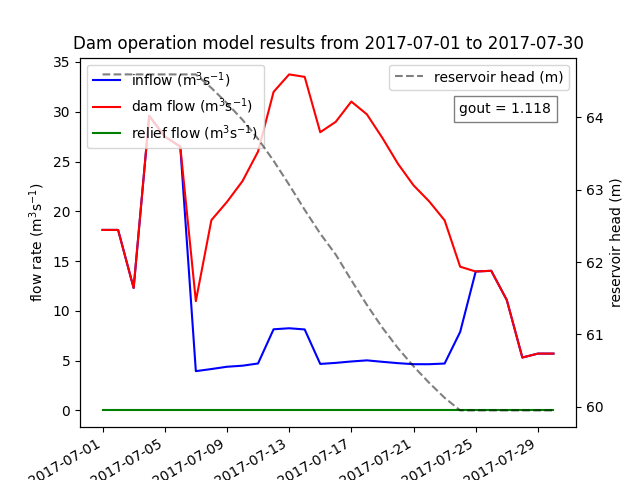
\includegraphics[width=0.45\textwidth]{2017-07-01-2017-07-30_optimization.png.png}}
\subfigure[1 month 2018]{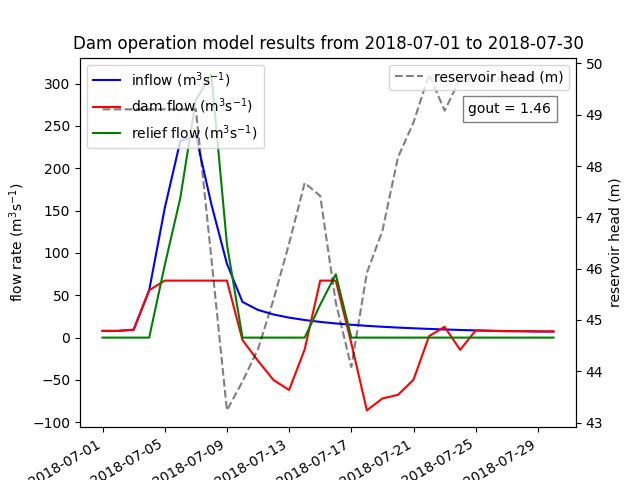
\includegraphics[width=0.45\textwidth]{2018-07-01-2018-07-30_optimization.png.png}}
\subfigure[2 months 2017]{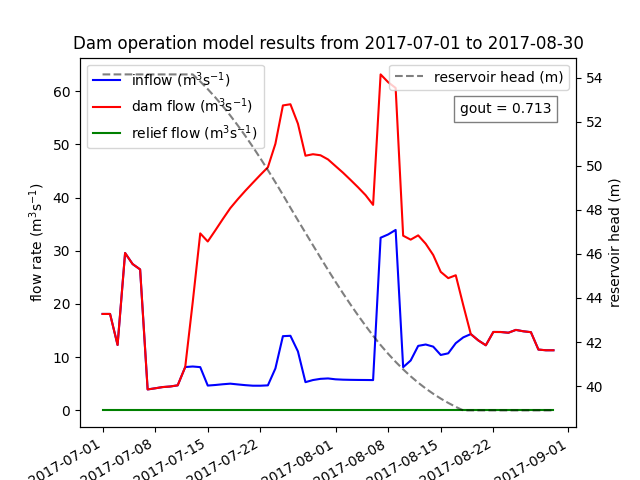
\includegraphics[width=0.45\textwidth]{2017-07-01-2017-08-30_optimization.png.png}}
\subfigure[2 months 2018]{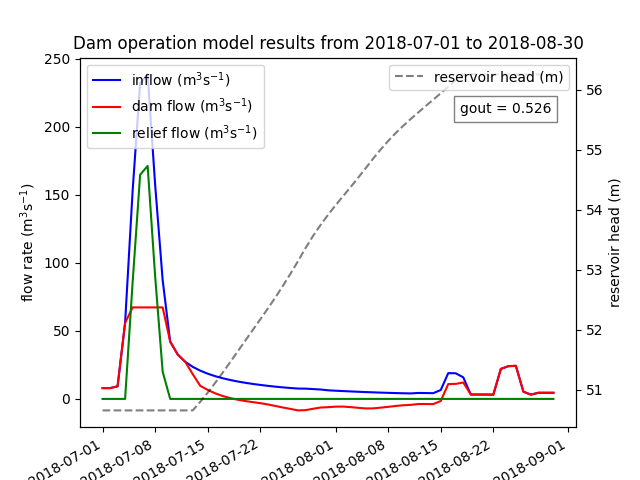
\includegraphics[width=0.45\textwidth]{2018-07-01-2018-08-30_optimization.png.png}}
\subfigure[3 months 2017]{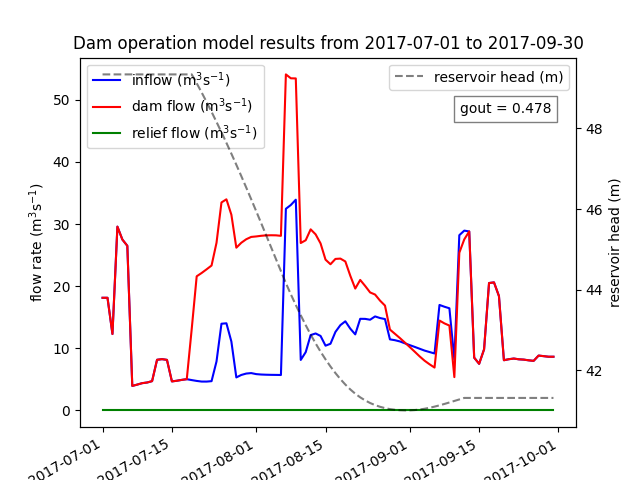
\includegraphics[width=0.45\textwidth]{2017-07-01-2017-09-30_optimization.png.png}}
\subfigure[3 months 2018]{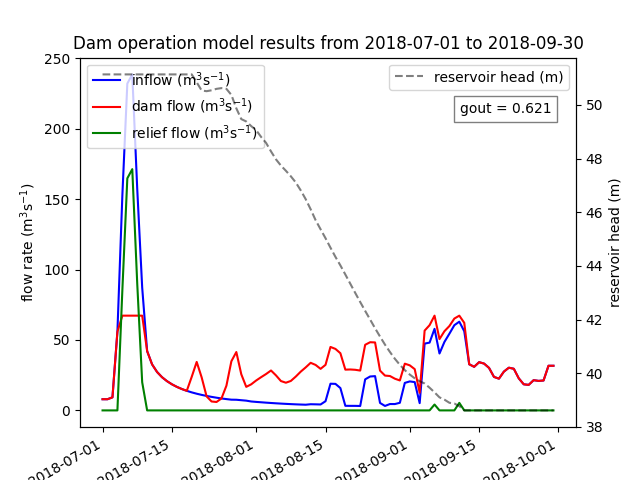
\includegraphics[width=0.45\textwidth]{2018-07-01-2018-09-30_optimization.png.png}}
\subfigure[4 months 2017]{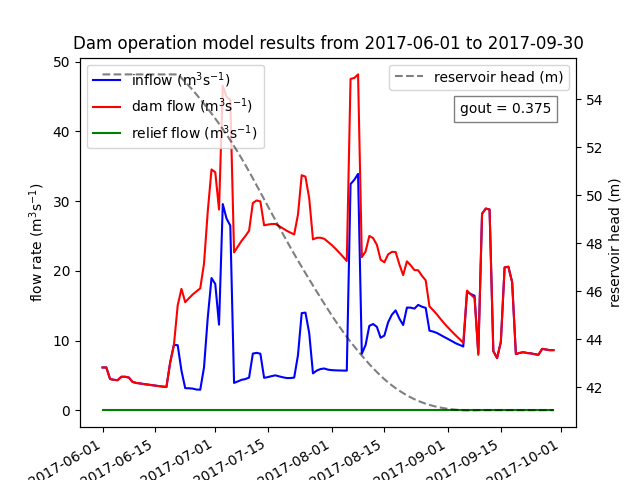
\includegraphics[width=0.45\textwidth]{2017-06-01-2017-09-30_optimization.png.png}}
\subfigure[4 months 2018]{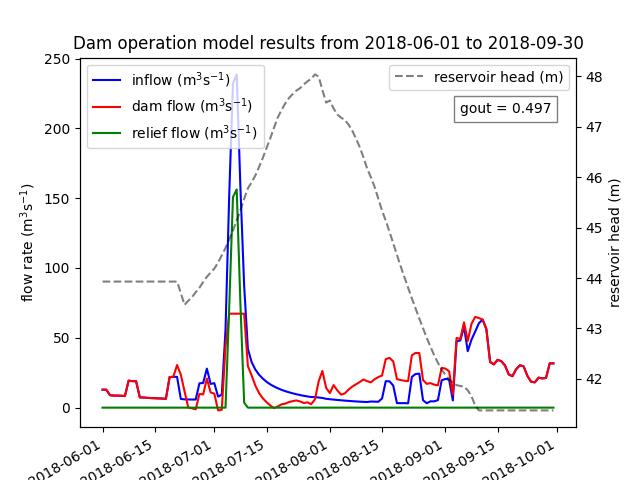
\includegraphics[width=0.45\textwidth]{2018-06-01-2018-09-30_optimization.png.png}}
\caption{Running the dam optimization model for a range of time periods in 2017 and 2018 using the default parameters. Note the different scales on the y-axes.}
\label{fig:Q1-varying-time-period}
\end{figure}


Generally, we find that the dam optimization model produces more plausible results for longer time periods of input data, ideally between 1-3 months. The 1 month results for 2017 and 2018 are shown in Figure \ref{fig:Q1-varying-time-period} (a) and (b) respectively. The 2018 run for July shown in figure \ref*{fig:Q1-varying-time-period}a shows significant variation in the reservoir head, with oscillations of 3m amplitude during mid-July. This seems unlikely, as such operational patterns would be challenging to manage over such short timescales, however, the occurence of extreme rainfall accumulations in late June (and early July) may necessitate such operational patterns. The optimization model appears to show plausible, stable solutions for the two month and three month periods shown in figures \ref*{fig:Q1-varying-time-period}c to \ref*{fig:Q1-varying-time-period}e; flow through the turbines (shown in red) follows the pattern of inflow (shown in blue) and the reservoir head (grey dashed line) shows a steady decrease (increase for 2 months in 2018, figure \ref*{fig:Q1-varying-time-period}d). The four month run for 2017, in figure \ref*{fig:Q1-varying-time-period}g, appears largely similar to the 3 month solution and generally appears stable. However, the four month solution for 2018 shows different characteristics to the the 2 and 3 month solution for the same year, in figure \ref*{fig:Q1-varying-time-period}h. The bell-shaped trend in reservoir head is plausible, due to the occurence of the rainfall event in early July, however the 4 month solution does not pick up the spikes in relief flow in early August (shown in figure \ref*{fig:Q1-varying-time-period}f) in the 3 month solution. False negatives, where the optimization model does not predict relief flow when needed, could be damaging due to risks of the dam overtopping and causing flooding. When provided with reanalyis data from ERA5 as input, the optimization model appears to perform best in the 1-3 months range.\\

\subsubsection*{Q2 - Optimization model sensitivity}

To assess the sensitivity of the optimization model to changes in the parameters, we run the model for different values of $W_{max}$, $H_{max}$, and $H_{min}$ for four months of 2017 (June, July, August and September).\\

% set up a figure with two columns and two rows
% top left is for the low tau plot
% top right is for the high tau plot
% bottom left is for the low range plot
% bottom right is for the high range plot

\begin{figure}
\centering
\subfigure[Low $\tau$]{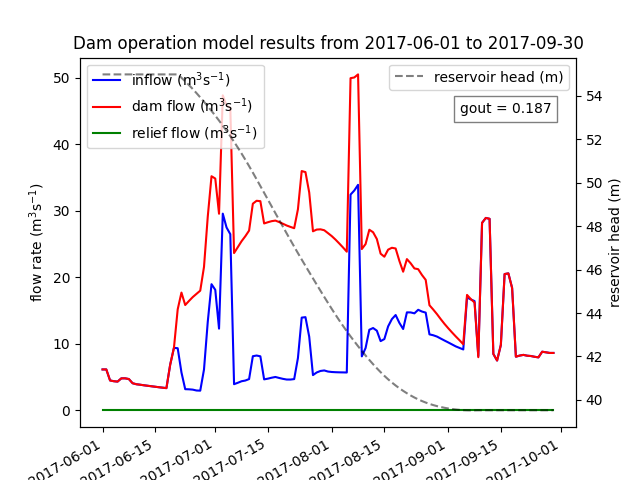
\includegraphics[width=0.45\textwidth]{2017-06-01-2017-09-30_optimization_Q2_Wmax_low_tau.png.png}}
\subfigure[High $\tau$]{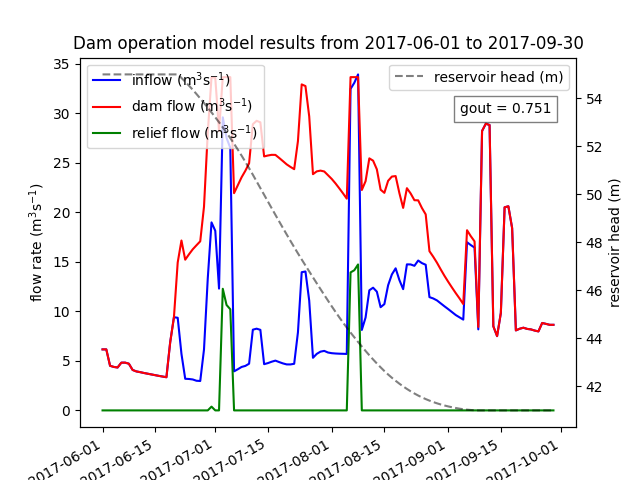
\includegraphics[width=0.45\textwidth]{2017-06-01-2017-09-30_optimization_Q2_Wmax_high_tau.png.png}}
\subfigure[Low range]{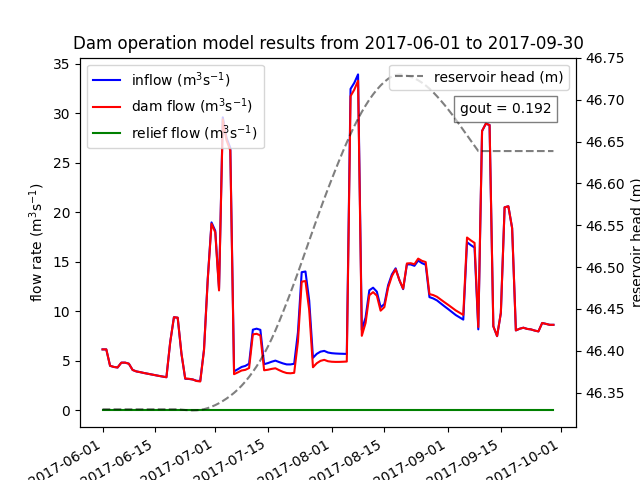
\includegraphics[width=0.45\textwidth]{2017-06-01-2017-09-30_optimization_Q2_small_range.png.png}}
\subfigure[High range]{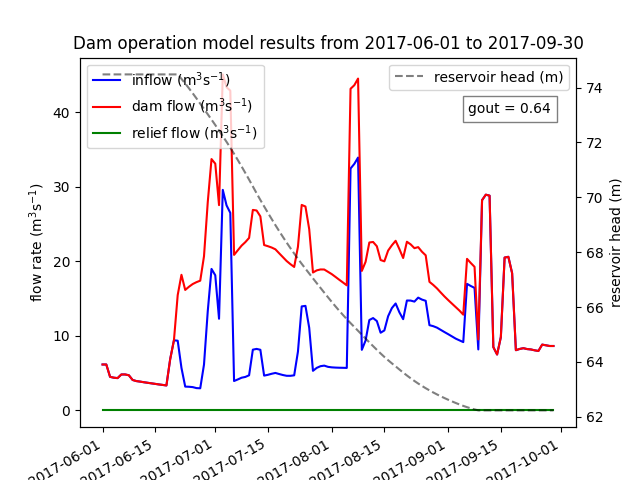
\includegraphics[width=0.45\textwidth]{2017-06-01-2017-09-30_optimization_Q2_large_range.png.png}}
\caption{Running the dam optimization model for four months of 2017 using different values of $W_{max}$, $H_{max}$, and $H_{min}$. A low value for $\tau$ results in a high $W_{max}$ and vice versa. Low range and high range of reservoir head are considered to assess the sensitivity of the model to changes in $H_{max}$ and $H_{min}$. Note the different scales of the y axes.}
\label{fig:Q2-sensitivity-to-params}
\end{figure}

Varying the value of $\tau$ changes the distribution of flow through the turbines and relief flow, as shown in figure \ref*{fig:Q2-sensitivity-to-params}a and \ref*{fig:Q2-sensitivity-to-params}b. With a high value for $\tau$ the maximum flow rate through the turbines ($W_{max}$) is reduced, which results in a higher proportion of the outflow being diverted to relief flow (total flow is diverted into relief flow when the $W_{max}$ threshold is exceeded). The optimization model produces more total outflow for the low $\tau$ (high $W_{max}$) case, shown by the range of reservoir head in figure \ref*{fig:Q2-sensitivity-to-params}a, as the model must optimize within tighter constraints ($W_{min} \leq W_n \leq W_{max}$) for the high $\tau$ (low $W_{max}$) case.\\

The sensitivity of the model to changes in $H_{max}$ and $H_{min}$ are shown in figures \ref*{fig:Q2-sensitivity-to-params}c and \ref*{fig:Q2-sensitivity-to-params}d respectively. For the low range case, the optimization model maintains the reservoir head within a narrow range of around 0.5m and produces flow through the turbines which appears tightly coupled to the inflow. As the model is subject to strict constraints for $H_n$, the model is limited in the solutions it can generate. For the high range case, the reservoir head varies more widely, with a range of around 10m, and the flow through the turbines distinct from the inflow. The model is less constrained by the $H_n$ constraints and is able to generate a wider range of solutions.\\

\subsubsection*{Q3 - Comparison of ERA5 and S2S data}

To evaluate the similarity of the two datasets, we compare the full field of runoff values from ERA5 and uncalibrated ECMWF subseasonal forecast data. The forecast data were preproccesed to convert the runoff rate per day (units: kg m$^{-2}$) to runoff in metres (ERA5 data); this processing is described in the methods section. The ERA5 data was downscaled to the same resolution as the S2S data (1.5$^{\circ}$) using the bilinear interpolation method. The runoff values are compared using a probability density function (PDF), shown in figure \ref*{fig:Q3-comparison-of-ERA5-and-S2S-data}.\\

% set up a single figure for the PDF comparison of uncalibrated S2S
% \begin{figure}
% \centering
% \scalebox{0.5}{\includegraphics{PDF_comparison_ERA5_S2S_uncalibrated.png}}
% \label{fig:Q3-comparison-of-ERA5-and-S2S-data}
% \caption{Comparison of the probability density function of ERA5 and uncalibrated S2S data. Mean and standard deviation of the two datasets are shown.}
% \end{figure}

% write this bit once the plots are sorted out
The most noticeable difference between the two datasets is the difference in interquartile range...

\subsubsection*{Q4 - Calibration of S2S data}

To calibrate the S2S data, we use the ERA5 data as a reference to adjust the variance of the S2S data. This calibration is performed according to equation (\ref{calibration}), without adjustment of the mean using $c_0$. Once again, the statistics of the two datasets are compared by using a PDF with the mean and interquartile range, in figure \ref*{Q4-comparison-of-calibrated-data}. \\



\section*{Discussion}

\section*{Summary}



% references don't seem to be working - sort this out later
\printbibliography

\end{document}

